\documentclass{article}\usepackage[]{graphicx}\usepackage[]{color}
%% maxwidth is the original width if it is less than linewidth
%% otherwise use linewidth (to make sure the graphics do not exceed the margin)
\makeatletter
\def\maxwidth{ %
  \ifdim\Gin@nat@width>\linewidth
    \linewidth
  \else
    \Gin@nat@width
  \fi
}
\makeatother

\definecolor{fgcolor}{rgb}{0.345, 0.345, 0.345}
\newcommand{\hlnum}[1]{\textcolor[rgb]{0.686,0.059,0.569}{#1}}%
\newcommand{\hlstr}[1]{\textcolor[rgb]{0.192,0.494,0.8}{#1}}%
\newcommand{\hlcom}[1]{\textcolor[rgb]{0.678,0.584,0.686}{\textit{#1}}}%
\newcommand{\hlopt}[1]{\textcolor[rgb]{0,0,0}{#1}}%
\newcommand{\hlstd}[1]{\textcolor[rgb]{0.345,0.345,0.345}{#1}}%
\newcommand{\hlkwa}[1]{\textcolor[rgb]{0.161,0.373,0.58}{\textbf{#1}}}%
\newcommand{\hlkwb}[1]{\textcolor[rgb]{0.69,0.353,0.396}{#1}}%
\newcommand{\hlkwc}[1]{\textcolor[rgb]{0.333,0.667,0.333}{#1}}%
\newcommand{\hlkwd}[1]{\textcolor[rgb]{0.737,0.353,0.396}{\textbf{#1}}}%
\let\hlipl\hlkwb

\usepackage{framed}
\makeatletter
\newenvironment{kframe}{%
 \def\at@end@of@kframe{}%
 \ifinner\ifhmode%
  \def\at@end@of@kframe{\end{minipage}}%
  \begin{minipage}{\columnwidth}%
 \fi\fi%
 \def\FrameCommand##1{\hskip\@totalleftmargin \hskip-\fboxsep
 \colorbox{shadecolor}{##1}\hskip-\fboxsep
     % There is no \\@totalrightmargin, so:
     \hskip-\linewidth \hskip-\@totalleftmargin \hskip\columnwidth}%
 \MakeFramed {\advance\hsize-\width
   \@totalleftmargin\z@ \linewidth\hsize
   \@setminipage}}%
 {\par\unskip\endMakeFramed%
 \at@end@of@kframe}
\makeatother

\definecolor{shadecolor}{rgb}{.97, .97, .97}
\definecolor{messagecolor}{rgb}{0, 0, 0}
\definecolor{warningcolor}{rgb}{1, 0, 1}
\definecolor{errorcolor}{rgb}{1, 0, 0}
\newenvironment{knitrout}{}{} % an empty environment to be redefined in TeX

\usepackage{alltt}
\IfFileExists{upquote.sty}{\usepackage{upquote}}{}
\begin{document}


\section{Data Processing}

\subsection{Create path temperature sensor csv files}

\begin{knitrout}
\definecolor{shadecolor}{rgb}{0.969, 0.969, 0.969}\color{fgcolor}\begin{kframe}
\begin{alltt}
\hlstd{filepath106} \hlkwb{=} \hlstr{"/home/CAMPUS/mwl04747/github/Climate_Change_Narratives/Data/FA19/Onset_Data/20724106.csv"}

\hlstd{filepath107} \hlkwb{=} \hlstr{"/home/CAMPUS/mwl04747/github/Climate_Change_Narratives/Data/FA19/Onset_Data/20724107.csv"}

\hlstd{filepath109} \hlkwb{=} \hlstr{"/home/CAMPUS/mwl04747/github/Climate_Change_Narratives/Data/FA19/Onset_Data/20724109.csv"}

\hlstd{filepath110} \hlkwb{=} \hlstr{"/home/CAMPUS/mwl04747/github/Climate_Change_Narratives/Data/FA19/Onset_Data/20724110.csv"}

\hlstd{filepath543} \hlkwb{=} \hlstr{"/home/CAMPUS/mwl04747/github/Climate_Change_Narratives/Data/FA19/Onset_Data/10998543.csv"}

\hlstd{filepath544} \hlkwb{=} \hlstr{"/home/CAMPUS/mwl04747/github/Climate_Change_Narratives/Data/FA19/Onset_Data/10998544.csv"}
\end{alltt}
\end{kframe}
\end{knitrout}

\subsection{Read csv files into R and clean files}

The headers are a mess, so I had to skip the first line before reading the CSV file. After that, I renamed the first few columns and then assigned the location from the header, manually. Total pain!

\begin{knitrout}
\definecolor{shadecolor}{rgb}{0.969, 0.969, 0.969}\color{fgcolor}\begin{kframe}
\begin{alltt}
\hlstd{onset106} \hlkwb{=} \hlkwd{read.csv}\hlstd{(filepath106,} \hlkwc{skip} \hlstd{=} \hlnum{1}\hlstd{);} \hlkwd{str}\hlstd{(onset106)}
\end{alltt}
\begin{verbatim}
## 'data.frame':	1881 obs. of  7 variables:
##  $ X.                                                                          : int  1 2 3 4 5 6 7 8 9 10 ...
##  $ Date.Time..GMT.08.00                                                        : Factor w/ 1881 levels "11/20/19 01:00:00 AM",..: 89 91 93 95 1 3 5 7 9 11 ...
##  $ Temp...F..LGR.S.N..20724106..SEN.S.N..20724106..LBL..Gandalf..Walker.Beach..: num  59.7 59.9 59.9 60 59.9 ...
##  $ Coupler.Attached..LGR.S.N..20724106..SEN.S.N..20724106.                     : Factor w/ 2 levels "","Logged": 1 1 1 1 1 1 1 1 1 1 ...
##  $ Host.Connected..LGR.S.N..20724106..SEN.S.N..20724106.                       : Factor w/ 2 levels "","Logged": 1 1 1 1 1 1 1 1 1 1 ...
##  $ Stopped..LGR.S.N..20724106..SEN.S.N..20724106.                              : Factor w/ 2 levels "","Logged": 1 1 1 1 1 1 1 1 1 1 ...
##  $ End.Of.File..LGR.S.N..20724106..SEN.S.N..20724106.                          : Factor w/ 2 levels "","Logged": 1 1 1 1 1 1 1 1 1 1 ...
\end{verbatim}
\begin{alltt}
\hlkwd{names}\hlstd{(onset106)} \hlkwb{=} \hlkwd{c}\hlstd{(}\hlstr{"Obs"}\hlstd{,} \hlstr{"DateTime"}\hlstd{,} \hlstr{"Temp"}\hlstd{)}
\hlstd{onset106}\hlopt{$}\hlstd{Location} \hlkwb{=} \hlstr{"Walker Beach"}\hlstd{; onset106}\hlopt{$}\hlstd{Exposure} \hlkwb{=} \hlstr{"Shade"}\hlstd{; onset106} \hlkwb{<-} \hlstd{onset106[,}\hlkwd{c}\hlstd{(}\hlnum{1}\hlstd{,}\hlnum{8}\hlstd{,} \hlnum{9}\hlstd{,} \hlnum{2}\hlstd{,}\hlnum{3}\hlstd{)];} \hlkwd{head}\hlstd{(onset106)}
\end{alltt}
\begin{verbatim}
##   Obs     Location Exposure             DateTime   Temp
## 1   1 Walker Beach    Shade 11/20/19 12:00:00 AM 59.680
## 2   2 Walker Beach    Shade 11/20/19 12:15:00 AM 59.851
## 3   3 Walker Beach    Shade 11/20/19 12:30:00 AM 59.851
## 4   4 Walker Beach    Shade 11/20/19 12:45:00 AM 60.024
## 5   5 Walker Beach    Shade 11/20/19 01:00:00 AM 59.851
## 6   6 Walker Beach    Shade 11/20/19 01:15:00 AM 59.680
\end{verbatim}
\begin{alltt}
\hlstd{onset107} \hlkwb{=} \hlkwd{read.csv}\hlstd{(filepath107,} \hlkwc{skip} \hlstd{=} \hlnum{1}\hlstd{);} \hlkwd{str}\hlstd{(onset107)}
\end{alltt}
\begin{verbatim}
## 'data.frame':	1881 obs. of  7 variables:
##  $ X.                                                                            : int  1 2 3 4 5 6 7 8 9 10 ...
##  $ Date.Time..GMT.08.00                                                          : Factor w/ 1881 levels "11/20/19 01:00:00 AM",..: 89 91 93 95 1 3 5 7 9 11 ...
##  $ Temp...F..LGR.S.N..20724107..SEN.S.N..20724107..LBL..Gertrude..Tranquada.Lot..: num  58.6 59 59.2 59.3 59.2 ...
##  $ Coupler.Attached..LGR.S.N..20724107..SEN.S.N..20724107.                       : Factor w/ 2 levels "","Logged": 1 1 1 1 1 1 1 1 1 1 ...
##  $ Host.Connected..LGR.S.N..20724107..SEN.S.N..20724107.                         : Factor w/ 2 levels "","Logged": 1 1 1 1 1 1 1 1 1 1 ...
##  $ Stopped..LGR.S.N..20724107..SEN.S.N..20724107.                                : Factor w/ 2 levels "","Logged": 1 1 1 1 1 1 1 1 1 1 ...
##  $ End.Of.File..LGR.S.N..20724107..SEN.S.N..20724107.                            : Factor w/ 2 levels "","Logged": 1 1 1 1 1 1 1 1 1 1 ...
\end{verbatim}
\begin{alltt}
\hlkwd{names}\hlstd{(onset107)} \hlkwb{=} \hlkwd{c}\hlstd{(}\hlstr{"Obs"}\hlstd{,} \hlstr{"DateTime"}\hlstd{,} \hlstr{"Temp"}\hlstd{)}
\hlstd{onset107}\hlopt{$}\hlstd{Location} \hlkwb{=} \hlstr{"Tranquada Lot"}\hlstd{; onset107}\hlopt{$}\hlstd{Exposure} \hlkwb{=} \hlstr{"Sun"}\hlstd{; onset107} \hlkwb{<-} \hlstd{onset107[,}\hlkwd{c}\hlstd{(}\hlnum{1}\hlstd{,}\hlnum{8}\hlstd{,} \hlnum{9}\hlstd{,} \hlnum{2}\hlstd{,}\hlnum{3}\hlstd{)];} \hlkwd{head}\hlstd{(onset107)}
\end{alltt}
\begin{verbatim}
##   Obs      Location Exposure             DateTime   Temp
## 1   1 Tranquada Lot      Sun 11/20/19 12:00:00 AM 58.647
## 2   2 Tranquada Lot      Sun 11/20/19 12:15:00 AM 58.993
## 3   3 Tranquada Lot      Sun 11/20/19 12:30:00 AM 59.164
## 4   4 Tranquada Lot      Sun 11/20/19 12:45:00 AM 59.337
## 5   5 Tranquada Lot      Sun 11/20/19 01:00:00 AM 59.164
## 6   6 Tranquada Lot      Sun 11/20/19 01:15:00 AM 59.164
\end{verbatim}
\begin{alltt}
\hlstd{onset109} \hlkwb{=} \hlkwd{read.csv}\hlstd{(filepath109,} \hlkwc{skip} \hlstd{=} \hlnum{1}\hlstd{);} \hlkwd{str}\hlstd{(onset109)}
\end{alltt}
\begin{verbatim}
## 'data.frame':	848 obs. of  4 variables:
##  $ X.                                                             : int  1 2 3 4 5 6 7 8 9 10 ...
##  $ Date.Time..GMT.08.00                                           : Factor w/ 848 levels "11/19/19 01:00:00 AM",..: 45 47 1 3 5 7 9 11 13 15 ...
##  $ Temp...F..LGR.S.N..20724109..SEN.S.N..20724109..LBL..KravisSun.: num  58.6 57.8 56.9 55.9 55.4 ...
##  $ End.Of.File..LGR.S.N..20724109..SEN.S.N..20724109.             : Factor w/ 2 levels "","Logged": 1 1 1 1 1 1 1 1 1 1 ...
\end{verbatim}
\begin{alltt}
\hlkwd{names}\hlstd{(onset109)} \hlkwb{=} \hlkwd{c}\hlstd{(}\hlstr{"Obs"}\hlstd{,} \hlstr{"DateTime"}\hlstd{,} \hlstr{"Temp"}\hlstd{)}
\hlstd{onset109}\hlopt{$}\hlstd{Location} \hlkwb{=} \hlstr{"Kravis"}\hlstd{; onset109}\hlopt{$}\hlstd{Exposure}\hlkwb{=}\hlstr{"Sun"}\hlstd{; onset109} \hlkwb{<-} \hlstd{onset109[,}\hlkwd{c}\hlstd{(}\hlnum{1}\hlstd{,}\hlnum{5}\hlstd{,}\hlnum{6}\hlstd{,} \hlnum{2}\hlstd{,}\hlnum{3}\hlstd{)];} \hlkwd{head}\hlstd{(onset109)}
\end{alltt}
\begin{verbatim}
##   Obs Location Exposure             DateTime   Temp
## 1   1   Kravis      Sun 11/19/19 12:00:00 AM 58.647
## 2   2   Kravis      Sun 11/19/19 12:30:00 AM 57.785
## 3   3   Kravis      Sun 11/19/19 01:00:00 AM 56.923
## 4   4   Kravis      Sun 11/19/19 01:30:00 AM 55.884
## 5   5   Kravis      Sun 11/19/19 02:00:00 AM 55.364
## 6   6   Kravis      Sun 11/19/19 02:30:00 AM 54.669
\end{verbatim}
\begin{alltt}
\hlstd{onset110} \hlkwb{=} \hlkwd{read.csv}\hlstd{(filepath110,} \hlkwc{skip} \hlstd{=} \hlnum{1}\hlstd{);} \hlkwd{str}\hlstd{(onset110)}
\end{alltt}
\begin{verbatim}
## 'data.frame':	1864 obs. of  7 variables:
##  $ X.                                                                          : int  1 2 3 4 5 6 7 8 9 10 ...
##  $ Date.Time..GMT.08.00                                                        : Factor w/ 1864 levels "11/20/19 01:00:00 AM",..: 89 91 93 95 1 3 5 7 9 11 ...
##  $ Temp...F..LGR.S.N..20724110..SEN.S.N..20724110..LBL..Gwen..SCC.Parking.Lot..: num  59.9 59.9 59.9 59.9 59.9 ...
##  $ Host.Connected..LGR.S.N..20724110..SEN.S.N..20724110.                       : Factor w/ 2 levels "","Logged": 1 1 1 1 1 1 1 1 1 1 ...
##  $ Coupler.Attached..LGR.S.N..20724110..SEN.S.N..20724110.                     : Factor w/ 2 levels "","Logged": 1 1 1 1 1 1 1 1 1 1 ...
##  $ Stopped..LGR.S.N..20724110..SEN.S.N..20724110.                              : Factor w/ 2 levels "","Logged": 1 1 1 1 1 1 1 1 1 1 ...
##  $ End.Of.File..LGR.S.N..20724110..SEN.S.N..20724110.                          : Factor w/ 2 levels "","Logged": 1 1 1 1 1 1 1 1 1 1 ...
\end{verbatim}
\begin{alltt}
\hlkwd{names}\hlstd{(onset110)} \hlkwb{=} \hlkwd{c}\hlstd{(}\hlstr{"Obs"}\hlstd{,} \hlstr{"DateTime"}\hlstd{,} \hlstr{"Temp"}\hlstd{)}
\hlstd{onset110}\hlopt{$}\hlstd{Location} \hlkwb{=} \hlstr{"SCC Parking Lot"}\hlstd{; onset110}\hlopt{$}\hlstd{Exposure} \hlkwb{=} \hlstr{"Shade"}\hlstd{; onset110} \hlkwb{<-} \hlstd{onset110[,}\hlkwd{c}\hlstd{(}\hlnum{1}\hlstd{,}\hlnum{8}\hlstd{,} \hlnum{9}\hlstd{,} \hlnum{2}\hlstd{,}\hlnum{3}\hlstd{)];} \hlkwd{head}\hlstd{(onset110)}
\end{alltt}
\begin{verbatim}
##   Obs        Location Exposure             DateTime   Temp
## 1   1 SCC Parking Lot    Shade 11/20/19 12:00:00 AM 59.851
## 2   2 SCC Parking Lot    Shade 11/20/19 12:15:00 AM 59.851
## 3   3 SCC Parking Lot    Shade 11/20/19 12:30:00 AM 59.851
## 4   4 SCC Parking Lot    Shade 11/20/19 12:45:00 AM 59.851
## 5   5 SCC Parking Lot    Shade 11/20/19 01:00:00 AM 59.851
## 6   6 SCC Parking Lot    Shade 11/20/19 01:15:00 AM 59.680
\end{verbatim}
\begin{alltt}
\hlstd{onset543} \hlkwb{=} \hlkwd{read.csv}\hlstd{(filepath543,} \hlkwc{skip} \hlstd{=} \hlnum{1}\hlstd{);} \hlkwd{str}\hlstd{(onset543)}
\end{alltt}
\begin{verbatim}
## 'data.frame':	981 obs. of  7 variables:
##  $ X.                                                                : int  1 2 3 4 5 6 7 8 9 10 ...
##  $ Date.Time..GMT.08.00                                              : Factor w/ 981 levels "11/19/19 01:00:00 AM",..: 45 47 1 3 5 7 9 11 13 15 ...
##  $ Temp...F..LGR.S.N..10998543..SEN.S.N..10998543..LBL..Sontag.Shade.: num  64.1 63.3 62.1 60.9 60.2 ...
##  $ Coupler.Attached..LGR.S.N..10998543..SEN.S.N..10998543.           : Factor w/ 2 levels "","Logged": 1 1 1 1 1 1 1 1 1 1 ...
##  $ Host.Connected..LGR.S.N..10998543..SEN.S.N..10998543.             : Factor w/ 2 levels "","Logged": 1 1 1 1 1 1 1 1 1 1 ...
##  $ Stopped..LGR.S.N..10998543..SEN.S.N..10998543.                    : Factor w/ 2 levels "","Logged": 1 1 1 1 1 1 1 1 1 1 ...
##  $ End.Of.File..LGR.S.N..10998543..SEN.S.N..10998543.                : Factor w/ 2 levels "","Logged": 1 1 1 1 1 1 1 1 1 1 ...
\end{verbatim}
\begin{alltt}
\hlkwd{names}\hlstd{(onset543)} \hlkwb{=} \hlkwd{c}\hlstd{(}\hlstr{"Obs"}\hlstd{,} \hlstr{"DateTime"}\hlstd{,} \hlstr{"Temp"}\hlstd{)}
\hlstd{onset543}\hlopt{$}\hlstd{Location} \hlkwb{=} \hlstr{"Sontag 1"}\hlstd{; onset543}\hlopt{$}\hlstd{Exposure} \hlkwb{=} \hlstr{"Sun"}\hlstd{; onset543} \hlkwb{<-} \hlstd{onset543[,}\hlkwd{c}\hlstd{(}\hlnum{1}\hlstd{,}\hlnum{8}\hlstd{,}\hlnum{9}\hlstd{,}\hlnum{2}\hlstd{,}\hlnum{3}\hlstd{)];} \hlkwd{head}\hlstd{(onset543)}
\end{alltt}
\begin{verbatim}
##   Obs Location Exposure             DateTime   Temp
## 1   1 Sontag 1      Sun 11/19/19 12:00:00 AM 64.139
## 2   2 Sontag 1      Sun 11/19/19 12:30:00 AM 63.282
## 3   3 Sontag 1      Sun 11/19/19 01:00:00 AM 62.083
## 4   4 Sontag 1      Sun 11/19/19 01:30:00 AM 60.883
## 5   5 Sontag 1      Sun 11/19/19 02:00:00 AM 60.195
## 6   6 Sontag 1      Sun 11/19/19 02:30:00 AM 60.195
\end{verbatim}
\begin{alltt}
\hlstd{onset544} \hlkwb{=} \hlkwd{read.csv}\hlstd{(filepath544,} \hlkwc{skip} \hlstd{=} \hlnum{1}\hlstd{);} \hlkwd{str}\hlstd{(onset544)}
\end{alltt}
\begin{verbatim}
## 'data.frame':	983 obs. of  8 variables:
##  $ X.                                                              : int  1 2 3 4 5 6 7 8 9 10 ...
##  $ Date.Time..GMT.08.00                                            : Factor w/ 983 levels "11/19/19 01:00:00 AM",..: 45 47 1 3 5 7 9 11 13 15 ...
##  $ Temp...F..LGR.S.N..10998544..SEN.S.N..10998544..LBL..Sontag.Sun.: num  64.1 62.9 61.7 61.6 60.5 ...
##  $ Coupler.Attached..LGR.S.N..10998544..SEN.S.N..10998544.         : Factor w/ 2 levels "","Logged": 1 1 1 1 1 1 1 1 1 1 ...
##  $ Host.Connected..LGR.S.N..10998544..SEN.S.N..10998544.           : Factor w/ 2 levels "","Logged": 1 1 1 1 1 1 1 1 1 1 ...
##  $ Coupler.Detached..LGR.S.N..10998544..SEN.S.N..10998544.         : Factor w/ 2 levels "","Logged": 1 1 1 1 1 1 1 1 1 1 ...
##  $ Stopped..LGR.S.N..10998544..SEN.S.N..10998544.                  : Factor w/ 2 levels "","Logged": 1 1 1 1 1 1 1 1 1 1 ...
##  $ End.Of.File..LGR.S.N..10998544..SEN.S.N..10998544.              : Factor w/ 2 levels "","Logged": 1 1 1 1 1 1 1 1 1 1 ...
\end{verbatim}
\begin{alltt}
\hlkwd{names}\hlstd{(onset544)} \hlkwb{=} \hlkwd{c}\hlstd{(}\hlstr{"Obs"}\hlstd{,} \hlstr{"DateTime"}\hlstd{,} \hlstr{"Temp"}\hlstd{)}
\hlstd{onset544}\hlopt{$}\hlstd{Location} \hlkwb{=} \hlstr{"Sontag 2"}\hlstd{; onset544}\hlopt{$}\hlstd{Exposure}\hlkwb{=}\hlstr{"Shade"}\hlstd{; onset544} \hlkwb{<-} \hlstd{onset544[,}\hlkwd{c}\hlstd{(}\hlnum{1}\hlstd{,}\hlnum{9}\hlstd{,}\hlnum{10}\hlstd{,} \hlnum{2}\hlstd{,}\hlnum{3}\hlstd{)];} \hlkwd{head}\hlstd{(onset544)}
\end{alltt}
\begin{verbatim}
##   Obs Location Exposure             DateTime   Temp
## 1   1 Sontag 2    Shade 11/19/19 12:00:00 AM 64.139
## 2   2 Sontag 2    Shade 11/19/19 12:30:00 AM 62.940
## 3   3 Sontag 2    Shade 11/19/19 01:00:00 AM 61.741
## 4   4 Sontag 2    Shade 11/19/19 01:30:00 AM 61.569
## 5   5 Sontag 2    Shade 11/19/19 02:00:00 AM 60.539
## 6   6 Sontag 2    Shade 11/19/19 02:30:00 AM 60.539
\end{verbatim}
\begin{alltt}
\hlstd{onset} \hlkwb{=} \hlkwd{rbind}\hlstd{(onset106, onset107, onset109, onset110, onset543, onset544)}
\end{alltt}
\end{kframe}
\end{knitrout}

\subsection{Fix Date-Time format}

I shouldn't be surprised, but the date/time format is not read correctly in R. So, after a bit of experimenting, I am using a package call \texttt{lubridate} that makes is a tiny bit easier.

\begin{knitrout}
\definecolor{shadecolor}{rgb}{0.969, 0.969, 0.969}\color{fgcolor}\begin{kframe}
\begin{alltt}
\hlstd{onset}\hlopt{$}\hlstd{Location}\hlkwb{=}\hlkwd{as.factor}\hlstd{(onset}\hlopt{$}\hlstd{Location)}
\hlcom{#str.date = as.character(onset$DateTime)}
\hlcom{#as.Date(str.date, format="%m%d%y", "h:m:s")}
\hlkwd{library}\hlstd{(}\hlstr{"lubridate"}\hlstd{)}
\end{alltt}


{\ttfamily\noindent\itshape\color{messagecolor}{\#\# \\\#\# Attaching package: 'lubridate'}}

{\ttfamily\noindent\itshape\color{messagecolor}{\#\# The following object is masked from 'package:base':\\\#\# \\\#\#\ \ \ \  date}}\begin{alltt}
\hlcom{#mdy_hms(str.date)}
\hlstd{onset}\hlopt{$}\hlstd{DateTime}\hlkwb{=}\hlstd{DateTime} \hlkwb{=} \hlkwd{mdy_hms}\hlstd{(onset}\hlopt{$}\hlstd{DateTime)}
\end{alltt}
\end{kframe}
\end{knitrout}

\subsection{Remove Data after Sensors were collected}

Although the sensors didn't start until we put them in the field, they did not stop until I downloaded the data. So, I manually removed the data based on a guess of when the temps did something odd for each site. 

\begin{knitrout}
\definecolor{shadecolor}{rgb}{0.969, 0.969, 0.969}\color{fgcolor}\begin{kframe}
\begin{alltt}
\hlcom{# Remove Data after Retrival}
\hlstd{onset2} \hlkwb{=} \hlkwd{subset}\hlstd{(onset,} \hlkwc{subset}\hlstd{=Location} \hlopt{==} \hlkwd{levels}\hlstd{(onset}\hlopt{$}\hlstd{Location)[}\hlnum{6}\hlstd{]} \hlopt{&} \hlstd{DateTime} \hlopt{<} \hlkwd{as.POSIXct}\hlstd{(}\hlstr{"2019-11-30 09:45:00"}\hlstd{,} \hlkwc{tz}\hlstd{=}\hlstr{"UTC"}\hlstd{))}
\hlstd{onset2} \hlkwb{=} \hlkwd{rbind}\hlstd{(onset2,} \hlkwd{subset}\hlstd{(onset,} \hlkwc{subset}\hlstd{=Location} \hlopt{==} \hlkwd{levels}\hlstd{(onset}\hlopt{$}\hlstd{Location)[}\hlnum{5}\hlstd{]} \hlopt{&} \hlstd{DateTime} \hlopt{<} \hlkwd{as.POSIXct}\hlstd{(}\hlstr{"2019-12-09 10:30:00"}\hlstd{,} \hlkwc{tz}\hlstd{=}\hlstr{"UTC"}\hlstd{)))}

\hlcom{# Sontag 2}
\hlstd{onset2} \hlkwb{=} \hlkwd{rbind}\hlstd{(onset2,} \hlkwd{subset}\hlstd{(onset,} \hlkwc{subset}\hlstd{=Location} \hlopt{==} \hlkwd{levels}\hlstd{(onset}\hlopt{$}\hlstd{Location)[}\hlnum{4}\hlstd{]} \hlopt{&} \hlstd{DateTime} \hlopt{<} \hlkwd{as.POSIXct}\hlstd{(}\hlstr{"2019-12-06 12:30:00"}\hlstd{,} \hlkwc{tz}\hlstd{=}\hlstr{"UTC"}\hlstd{)))}

\hlcom{# Sontag 1}
\hlstd{onset2} \hlkwb{=} \hlkwd{rbind}\hlstd{(onset2,} \hlkwd{subset}\hlstd{(onset,} \hlkwc{subset}\hlstd{=Location} \hlopt{==} \hlkwd{levels}\hlstd{(onset}\hlopt{$}\hlstd{Location)[}\hlnum{3}\hlstd{]} \hlopt{&} \hlstd{DateTime} \hlopt{<} \hlkwd{as.POSIXct}\hlstd{(}\hlstr{"2019-12-06 12:30:00"}\hlstd{,} \hlkwc{tz}\hlstd{=}\hlstr{"UTC"}\hlstd{)))}
\hlcom{# SCC Parking Lot}
\hlstd{onset2} \hlkwb{=} \hlkwd{rbind}\hlstd{(onset2,} \hlkwd{subset}\hlstd{(onset,} \hlkwc{subset}\hlstd{=Location} \hlopt{==} \hlkwd{levels}\hlstd{(onset}\hlopt{$}\hlstd{Location)[}\hlnum{2}\hlstd{]} \hlopt{&} \hlstd{DateTime} \hlopt{<} \hlkwd{as.POSIXct}\hlstd{(}\hlstr{"2019-12-07 14:30:00"}\hlstd{,} \hlkwc{tz}\hlstd{=}\hlstr{"UTC"}\hlstd{)))}
\hlcom{# Kravis Sun}
\hlstd{onset2} \hlkwb{=} \hlkwd{rbind}\hlstd{(onset2,} \hlkwd{subset}\hlstd{(onset,} \hlkwc{subset}\hlstd{=Location} \hlopt{==} \hlkwd{levels}\hlstd{(onset}\hlopt{$}\hlstd{Location)[}\hlnum{1}\hlstd{]} \hlopt{&} \hlstd{DateTime} \hlopt{<} \hlkwd{as.POSIXct}\hlstd{(}\hlstr{"2019-12-06 14:00:00"}\hlstd{,} \hlkwc{tz}\hlstd{=}\hlstr{"UTC"}\hlstd{)))}
\end{alltt}
\end{kframe}
\end{knitrout}

\section{Results}

\subsection{Interogating the Results}

First, we'll put everything in one graph (Figure~\ref{fig.alldatat}).

\begin{figure}
\caption{All time series in one graphic. Not easy to see what's going on.}
\label{fig.alldatat}

\begin{knitrout}
\definecolor{shadecolor}{rgb}{0.969, 0.969, 0.969}\color{fgcolor}\begin{kframe}
\begin{verbatim}
## [1] "Kravis"          "SCC Parking Lot" "Sontag 1"        "Sontag 2"       
## [5] "Tranquada Lot"   "Walker Beach"
\end{verbatim}
\end{kframe}
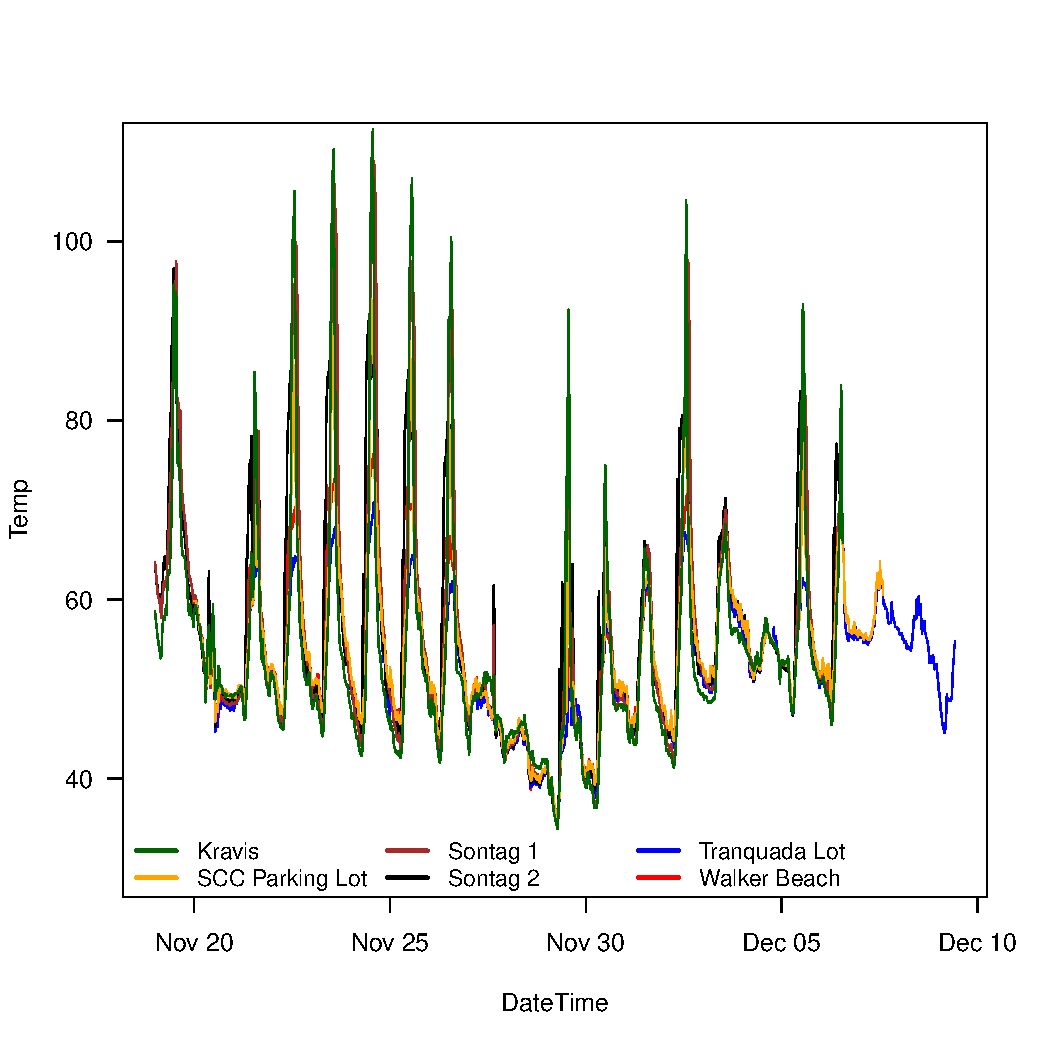
\includegraphics[width=\maxwidth]{figure/unnamed-chunk-5-1} 

\end{knitrout}
\end{figure}



\end{document}
